\section{Assignment 3: Scale-Invariant Blob Detection}
\label{sec:assignment3}

This assignment is about locating blobs of different sizes in images. A Laplacian blob detector is implemented and used in a scale-invariant way by convolving it with repeatedly blurred versions of the image to be analyzed.

\subsection{Problem definition}

Given an image, the problem is to find blob-like features of varying scale. In specific, the goals are to:
\begin{itemize}[noitemsep]
\item Implement a Laplacian of Gaussian (LoG) blob detector
\item Apply it to a reference image (\texttt{butterfly.jpg}) and an image of choice. Also apply it to half-sized versions of the images
\item Indicate the found blobs by overlaying circles, with the circle radii being representative of the found blob's size
\item Plot the LoG response over all scales at a specific keypoint for both the original and half-sized image
\item Discuss the results
\end{itemize}

\subsection{Methodology}

Todo ...

\subsection{Experiments}

Todo ...

\begin{figure}[h]
	\centering
	\begin{tabular}{cc}
		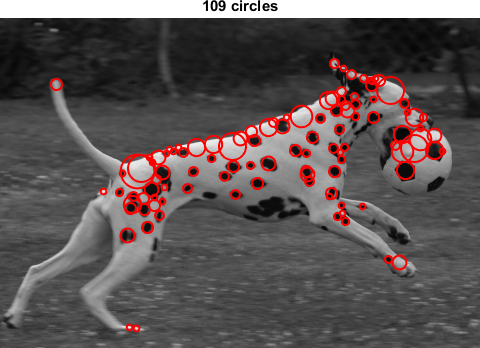
\includegraphics[width=0.5\textwidth]{figures/a3_dalmation_k020_full.png} &
		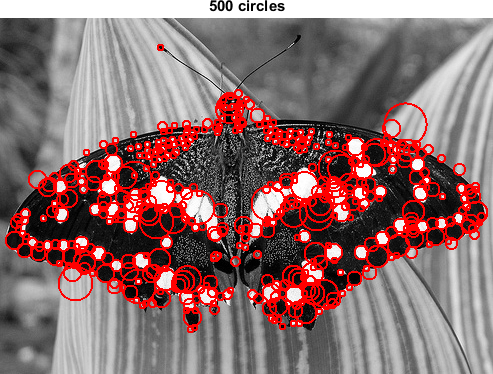
\includegraphics[width=0.5\textwidth]{figures/a3_butterfly_k020.png} \\
		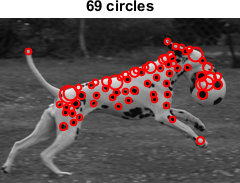
\includegraphics[width=0.25\textwidth]{figures/a3_dalmation_k020_half.png} &
		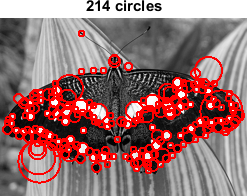
\includegraphics[width=0.25\textwidth]{figures/a3_butterfly_k020_small.png} \\
	\end{tabular}
	\caption{LoG blob detector applied to two different images and to half-sized versions of them. Parameters: $\sigma_0=2, k=1.25, threshold=0.20, levels=10$.}
	\label{fig:a3:thresholds}
\end{figure}

\begin{figure}[h]
	\centering
	\begin{tabular}{cc}
	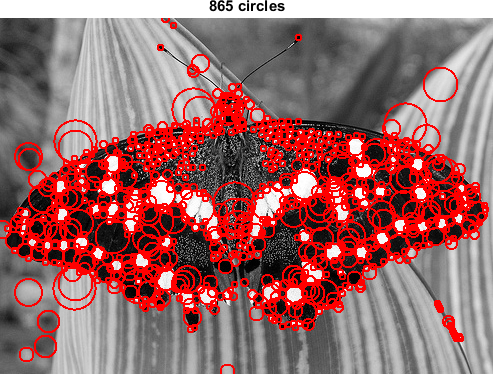
\includegraphics[width=0.4\textwidth]{figures/a3_butterfly_k015.png} &
	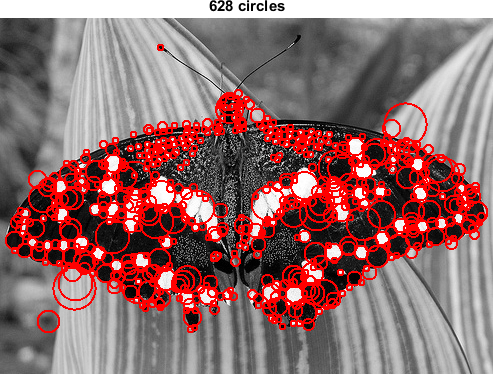
\includegraphics[width=0.4\textwidth]{figures/a3_butterfly_k018.png} \\
	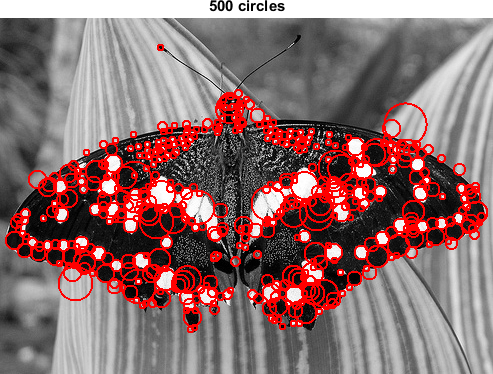
\includegraphics[width=0.4\textwidth]{figures/a3_butterfly_k020.png} &
	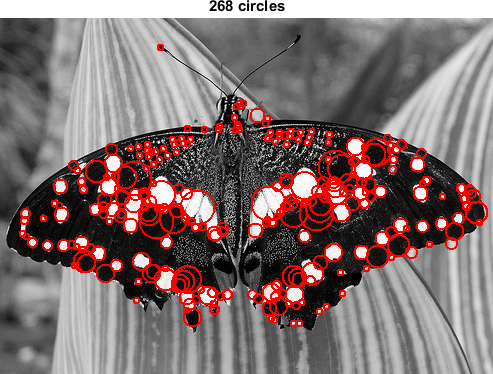
\includegraphics[width=0.4\textwidth]{figures/a3_butterfly_k025.png} \\
	\end{tabular}
	\caption{Illustration of the effect of different thresholds $t$. Top left: $t=0.15$. Top right: $t=0.18$. Bottom left: $t=0.20$. Bottom right: $t=0.25$.}
	\label{fig:a3:thresholds}
\end{figure}

\begin{figure}[h]
	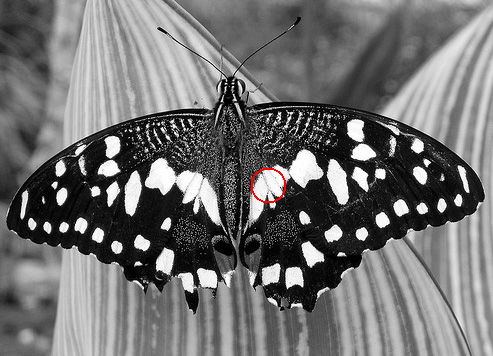
\includegraphics[width=0.5\textwidth]{figures/a3_butterfly_keypoint.png}
	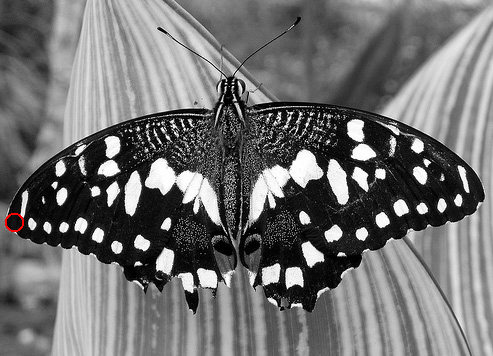
\includegraphics[width=0.5\textwidth]{figures/a3_butterfly_keypoint_2.png}
	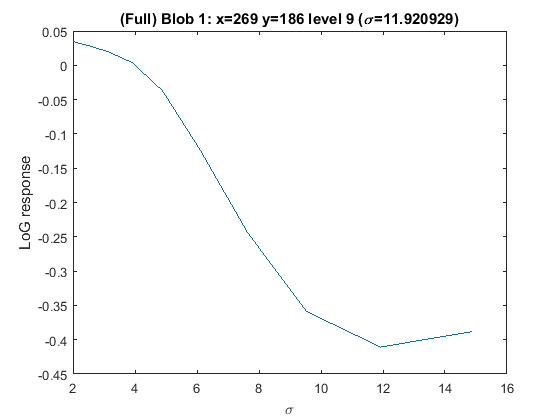
\includegraphics[width=0.5\textwidth]{figures/a3_butterfly_log_full.png}
	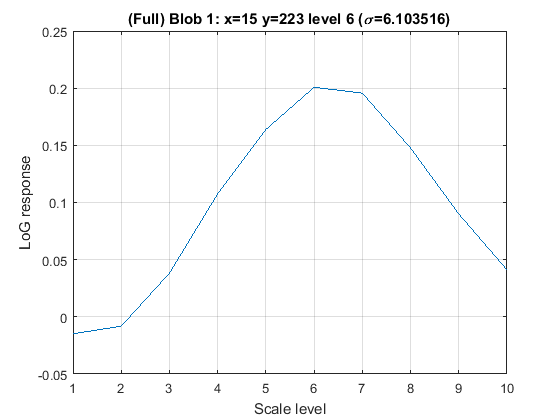
\includegraphics[width=0.5\textwidth]{figures/a3_butterfly_log_full_2.png}
	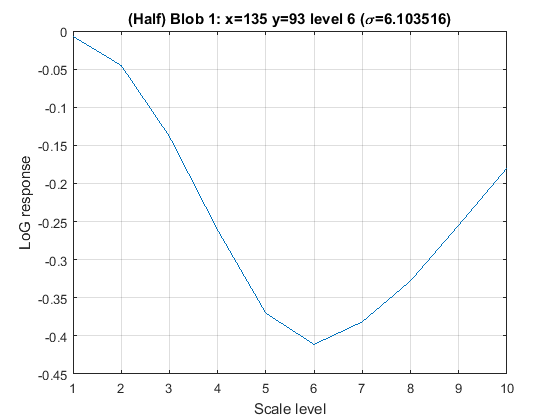
\includegraphics[width=0.5\textwidth]{figures/a3_butterfly_log_half.png}
	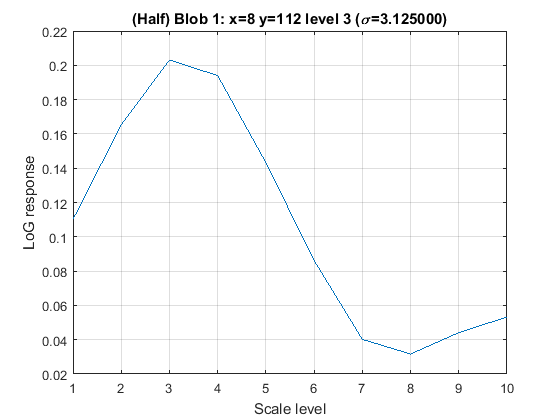
\includegraphics[width=0.5\textwidth]{figures/a3_butterfly_log_half_2.png}
	\caption{LoG response for two selected keypoints. The top row shows the chosen keypoint, the second and third rows show the LoG response for the full-sized and half-sized image. Left: A white-on-black blob (negative LoG response), right: a black-on-white blob (positive LoG response).}
	\label{fig:a3:logresponse}
\end{figure}


\subsection{Discussion}

Todo ...
